\subsubsection{Varying partition, source and destination sizes, keeping the same sources/destination ratio}

\begin{figure*}[!htbp]
        \centering
        \begin{subfigure}[b]{0.32\textwidth}
                \includegraphics[width=\textwidth]{figures/constantr_3.pdf}
                \caption{Disjoint}
                \label{fig:constantr_3}
        \end{subfigure}%
        ~ %add desired spacing between images, e. g. ~, \quad, \qquad, \hfill etc.
          %(or a blank line to force the subfigure onto a new line)
        \begin{subfigure}[b]{0.32\textwidth}
                \includegraphics[width=\textwidth]{figures/constantr_27}
                \caption{Overlap}
                \label{fig:constantr_27}
        \end{subfigure}
        ~ %add desired spacing between images, e. g. ~, \quad, \qquad, \hfill etc.
          %(or a blank line to force the subfigure onto a new line)
        \begin{subfigure}[b]{0.32\textwidth}
                \includegraphics[width=\textwidth]{figures/constantr_87}
                \caption{Subset}
                \label{fig:constantr_87}
        \end{subfigure}
        \caption{Varying the number of sources and destinations and total number of nodes while keeping the ratio constant (1:8).}
        \label{fig:constantr}
\end{figure*}

\begin{table*}[!htbp]
   \centering
    \begin{tabular}{| l | l | r | r | p{0.5cm} | p{0.5cm} | p{0.5cm} | p{0.5cm} |p{0.5cm} | p{0.5cm} |p{0.5cm} | p{0.5cm} |p{0.5cm} | p{0.5cm} |}
    \hline
    \multirow{3}{*}{Pattern} & \multirow{3}{*}{Type} & \multirow{3}{1cm}{BW (GB/s)} & \multicolumn{3}{ c| }{Num. of Paths} & \multicolumn{2}{ c| }{Hopbytes} & \multicolumn{2}{ c| }{Num of copies}& \multicolumn{2}{ c| }{Num of paths} & \multicolumn{2}{ c| }{Total data} \\ \cline{4-6}
    & & & \multirow{2}{0.5cm}{Total Paths} & \multicolumn{2}{ c| }{Per Job} & \multicolumn{2}{ c| }{Per Path (MB)} & \multicolumn{2}{ c| }{Per Path}& \multicolumn{2}{ c| }{Per Link}& \multicolumn{2}{ c| }{Per Link (MB)} \\ \cline{5-14}
    & & & & {Max} & Avg & Max & Avg & Max & Avg & Max & Avg & Max & Avg\\ \hline
    \multirow{3}{*}{Disjont} & OPT    & 188.62 & 1,169 & 6 & 2.28 & 83.88 & 23.02 & 1152 & 295.22 & 11 & 2.53 & 18.28 & 9.26 \\ \cline{2-14}
    & HEU 16 & 74.88  & 3,146 & 23 & 6.14 & 83.88 & 8.45 & 1152 & 108.24 & 16 & 4.94 & 63.04 & 6.92 \\ \cline{2-14}
    & MPI    & 45.18  & 512  & 1 & 1.00 & 92.27 & 50.33 & & & 16 & 3.07 & 134.21 & 25.76\\ \hline
    \multirow{3}{*}{Overlap} & OPT    & 200.03 & 1303 & 6 & 2.54 & 83.88 & 19.28  & 1152 & 243.96 & 13 & 2.74 & 16.97 & 9.04\\ \cline{2-14}
    & HEU 16 & 113.17  & 3273 & 26 & 6.39 & 75.49 & 7.41 & 1024 & 93.07 & 16 & 5.17 & 38.66 & 7.04 \\ \cline{2-14}
    & MPI    & 42.84 & 512 & 1 & 1.00 & 83.88 & 42.99 &  & & 16 & 3.38 & 134.21 & 28.36 \\ \hline
    \multirow{3}{*}{Subset} & OPT    & 199.20 & 1269 & 6 & 2.48 & 75.49 & 19.48 & 1024 & 245.66 & 11 & 2.79 & 17.10 & 9.32 \\ \cline{2-14}
    & HEU 16 &  61.71 & 3238 & 26 & 6.32 & 75.49 & 7.43 & 1024 & 93.22 & 16 & 5.28 & 45.08  & 7.35 \\ \cline{2-14}
    & MPI    &  41.37 & 512  & 1 & 1.00 & 83.88 &  41.94 & & & 16 & 3.52 & 134.21 & 29.49 \\ \hline
    \end{tabular}
    \caption{Throughput, total num of paths, number of paths per job, maximum and average values of hopbytes, number of copies, number of paths per link and amount of data per link for 3 patterns in 1024 nodes experiments.}
    \label{table:constantr}
\end{table*}

\begin{figure}[!htb]
\vspace{-0.1in}
\centering
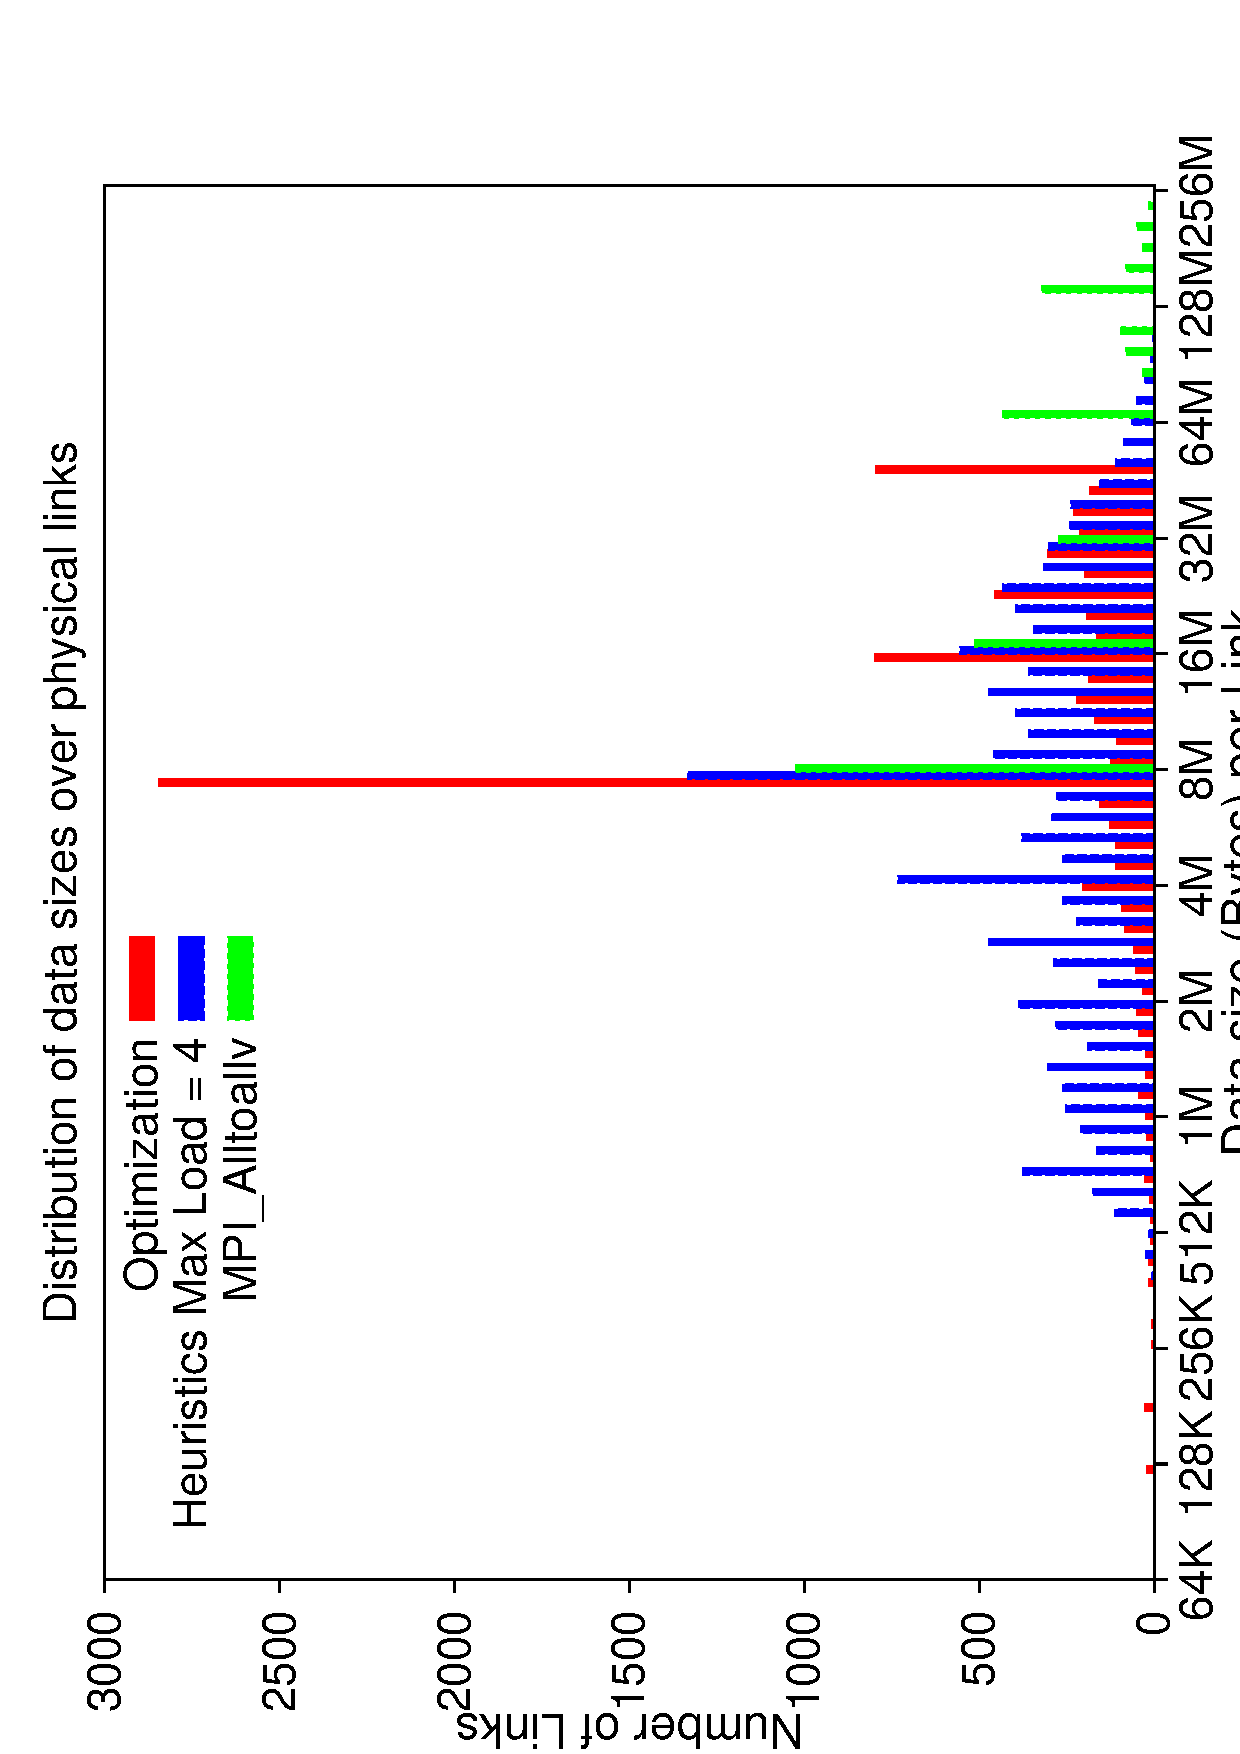
\includegraphics[scale=0.30]{figures/loaddata_histo.pdf}
\vspace{-0.1in}
\caption{Distribution of total amount of data per link for Disjoint pattern in 1024-node partition.}
\vspace{-0.1in}
\label{fig:loaddata_histo}
\end{figure}

\begin{figure}[!htb]
\vspace{-0.1in}
\centering
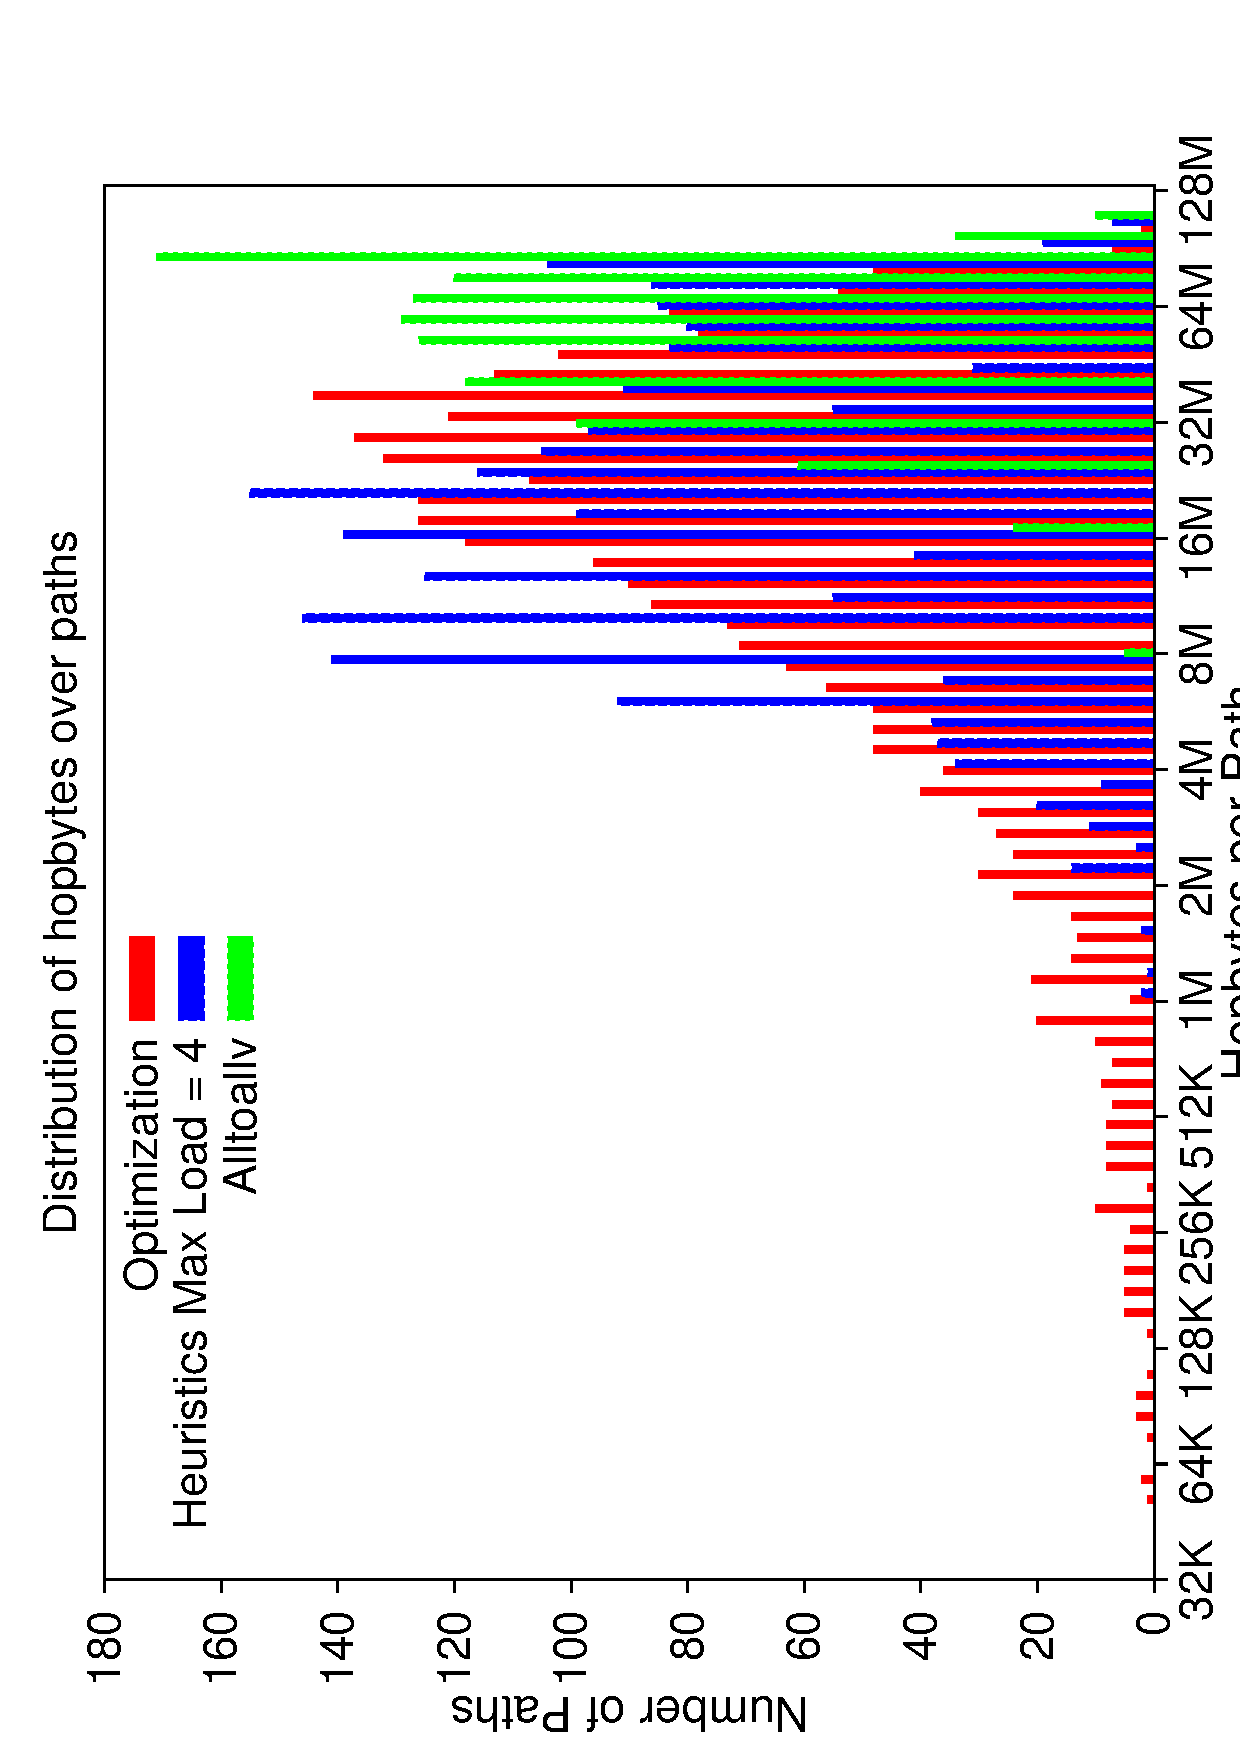
\includegraphics[scale=0.30]{figures/hopbyte_histo.pdf}
\vspace{-0.1in}
\caption{Distribution of hopbytes per path for Disjoint pattern in 1024-node partition.}
\vspace{-0.1in}
\label{fig:hopbyte_histo}
\end{figure}

In this experiment we vary the number of sources and destinations together with total number of nodes while keeping the ratio between the number of sources and destination at 1/8. While the total number of nodes P  increases from 512 to 8192 the first P/16 nodes send data to the last P/2 nodes. Each source has 8 destinations e.g node 0 sends data to nodes P/2, P/2+1, ...P/2+7. We tested the framework for 3 patterns: subset, disjoint and overlap, with 3 approaches of transferring data OPTIQ Optimization, OPTIQ Heuristics and MPI\_Alltoallv. We use 1 MPI/PAMI rank/node. The data size is 8 MB per pair. We set the $maxload$ to 16 for the Heuristic approach.

As shown in Figure \ref{fig:constantr} the Optimization approach has the highest throughput, the Heuristics approach is next and MPI\_Alltoall achieved the lowest throughput. The Table \ref{table:constantr} shows that in all three patterns the Heuristic with $maxload$ set to 16 was able to find highest number of paths. The Heurisc approach also has the highest maximum and average number paths for a job. As data is divided equally among paths, this led to lowest maximum and average values for hopbytes, number of copies per path. However this led to higher number of paths per physical link, and higher amount of data per physical link in the Heuristic approach in comparison to the Optimization approach. In Optimization the data is split among the paths to balance the amount of data between physical links, thus it has the lowest maximum amount of data per physical link. The distribution of the total amount of data in Figure \ref{fig:loaddata_histo} also shows this effect. This led to its highest throughput. MPI\_Alltoall approach has the lowest number of paths. With 1 path per pair of communication, data is not split. Thus it has the the highest hopbytes per path and amount of data per physical link. The distribution of its total data size per link in Figure \ref{fig:loaddata_histo} and its hopbytes per paths in Figure \ref{fig:hopbyte_histo} also show the effects. Both factors led to its lowest throughput.
